% Editable vector schematic of the completed native-JAX raw19 SAE experiment.
% Sources: encoder_chemistry_sae.py, modal_encoder_chemistry_sae_causal.py,
% trained_sae.json, chemical_features.json and causal manifests.
\documentclass[tikz,border=0pt]{standalone}
\usepackage{fontspec}
\setsansfont{LiberationSans}[Path=../../shared/assets/,Extension=.ttf,UprightFont=*-Regular,BoldFont=*-Bold]
\usepackage{amsmath}
\usepackage{unicode-math}
\setmathfont{Latin Modern Math}
\usetikzlibrary{arrows.meta,calc}
\definecolor{ink}{HTML}{0C0C0C}
\definecolor{muted}{HTML}{63676B}
\definecolor{accent}{HTML}{007C83}
\definecolor{control}{HTML}{A36F23}
\definecolor{lightfill}{HTML}{EDF6F5}
\hyphenpenalty=10000\exhyphenpenalty=10000
\begin{document}
\ifdefined\SlideDiagram
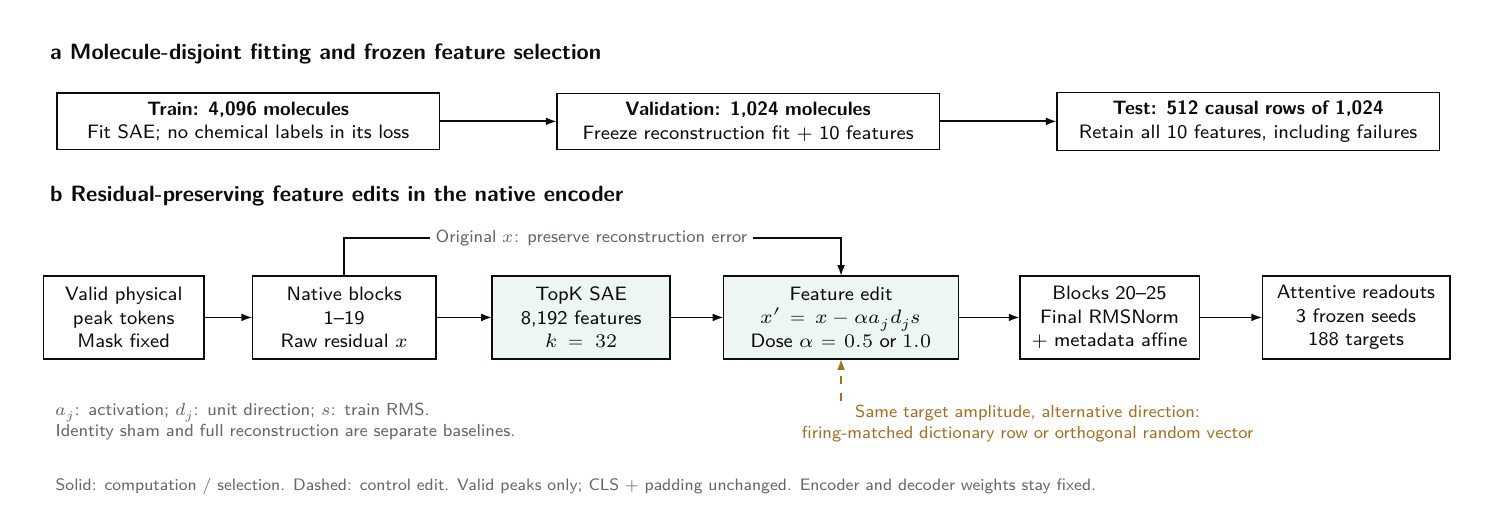
\begin{tikzpicture}[x=1cm,y=1cm,
 every node/.style={font=\sffamily\fontsize{7}{8.5}\selectfont,text=ink,align=center,inner sep=3pt,outer sep=0pt},
 box/.style={draw=ink,line width=.55pt,minimum height=1.05cm},
 flow/.style={-{Latex[length=1.4mm,width=1mm]},line width=.65pt,draw=ink},
 patch/.style={-{Latex[length=1.4mm,width=1mm]},line width=.65pt,draw=control,dashed},
 note/.style={font=\sffamily\fontsize{6.3}{7.6}\selectfont,text=muted},
 panel/.style={anchor=west,font=\sffamily\bfseries\fontsize{8}{10}\selectfont}]
\path[use as bounding box] (0,0) rectangle (18.3,6.05);
\node[panel] at (.18,5.72) {a  Molecule-disjoint fitting and frozen feature selection};
\node[box,text width=4.65cm,minimum height=.7cm] (str) at (2.8,4.86)
 {\textbf{Train: 4,096 molecules}\\Fit SAE; no chemical labels in its loss};
\node[box,text width=4.65cm,minimum height=.7cm] (sva) at (9.15,4.86)
 {\textbf{Validation: 1,024 molecules}\\Freeze reconstruction fit + 10 features};
\node[box,text width=4.65cm,minimum height=.7cm] (ste) at (15.5,4.86)
 {\textbf{Test: 512 causal rows of 1,024}\\Retain all 10 features, including failures};
\draw[flow] (str.east)--(sva.west);
\draw[flow] (sva.east)--(ste.west);
\node[panel] at (.18,3.91) {b  Residual-preserving feature edits in the native encoder};
\node[box,text width=1.83cm] (sp) at (1.22,2.37)
 {Valid physical\\peak tokens\\Mask fixed};
\node[box,text width=2.12cm] (se) at (4.02,2.37)
 {Native blocks\\1--19\\Raw residual $x$};
\node[box,text width=2.05cm,fill=lightfill] (ss) at (7.03,2.37)
 {TopK SAE\\8,192 features\\$k=32$};
\node[box,text width=2.77cm,fill=lightfill] (si) at (10.33,2.37)
 {Feature edit\\$x'=x-\alpha a_j d_j s$\\Dose $\alpha=0.5$ or $1.0$};
\node[box,text width=2.07cm] (sr) at (13.74,2.37)
 {Blocks 20--25\\Final RMSNorm\\+ metadata affine};
\node[box,text width=2.17cm] (sh) at (16.87,2.37)
 {Attentive readouts\\3 frozen seeds\\188 targets};
\draw[flow] (sp.east)--(se.west);
\draw[flow] (se.east)--(ss.west);
\draw[flow] (ss.east)--(si.west);
\draw[flow] (si.east)--(sr.west);
\draw[flow] (sr.east)--(sh.west);
\draw[flow] (se.north)--(4.02,3.38)--(10.33,3.38)--(si.north);
\node[note,fill=white,inner sep=2pt] at (7.16,3.38) {Original $x$: preserve reconstruction error};
\node[note,anchor=west,text width=6.5cm,align=left] at (.25,1.05)
 {$a_j$: activation; $d_j$: unit direction; $s$: train RMS.\\Identity sham and full reconstruction are separate baselines.};
\node[note,text=control,text width=10.5cm] (sc) at (12.7,1.02)
 {Same target amplitude, alternative direction:\\firing-matched dictionary row or orthogonal random vector};
\draw[patch] (10.33,1.31)--(si.south);
\node[anchor=west,note,font=\sffamily\fontsize{6}{7.2}\selectfont] at (.25,.23)
 {Solid: computation / selection. Dashed: control edit. Valid peaks only; CLS + padding unchanged. Encoder and decoder weights stay fixed.};
\end{tikzpicture}
\else
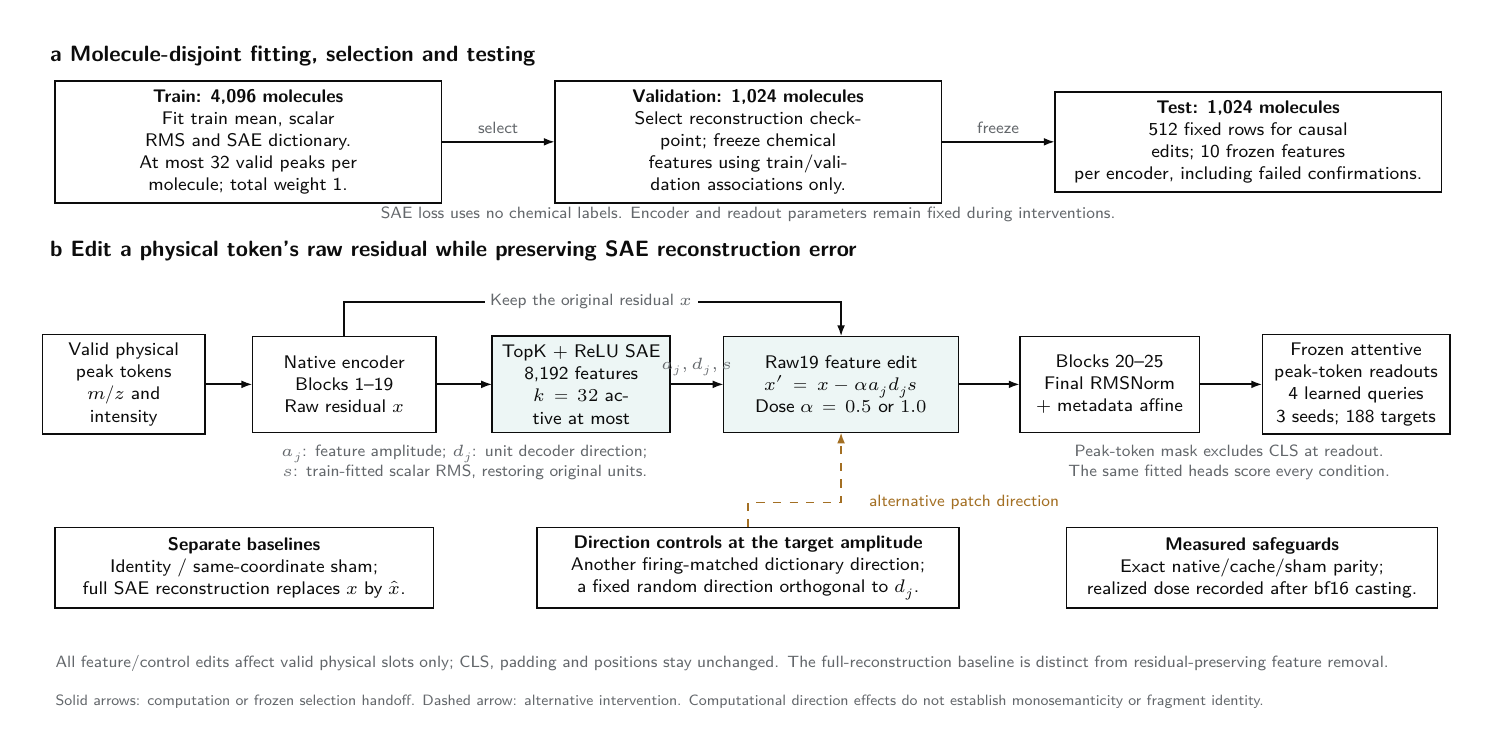
\begin{tikzpicture}[x=1cm,y=1cm,
 every node/.style={font=\sffamily\fontsize{6.6}{8}\selectfont,text=ink,align=center,inner sep=3pt,outer sep=0pt},
 box/.style={draw=ink,line width=.55pt,minimum height=1.22cm},
 flow/.style={-{Latex[length=1.4mm,width=1mm]},line width=.65pt,draw=ink},
 patch/.style={-{Latex[length=1.4mm,width=1mm]},line width=.65pt,draw=control,dashed},
 note/.style={font=\sffamily\fontsize{5.9}{7.2}\selectfont,text=muted},
 panel/.style={anchor=west,font=\sffamily\bfseries\fontsize{8}{10}\selectfont}]
\path[use as bounding box] (0,0) rectangle (18.3,8.8);
\node[panel] at (.18,8.44) {a  Molecule-disjoint fitting, selection and testing};
\node[box,text width=4.7cm,minimum height=1.1cm] (train) at (2.8,7.35)
 {\textbf{Train: 4,096 molecules}\\Fit train mean, scalar RMS and SAE dictionary.\\At most 32 valid peaks per molecule; total weight 1.};
\node[box,text width=4.7cm,minimum height=1.1cm] (val) at (9.15,7.35)
 {\textbf{Validation: 1,024 molecules}\\Select reconstruction checkpoint; freeze chemical\\features using train/validation associations only.};
\node[box,text width=4.7cm,minimum height=1.1cm] (test) at (15.5,7.35)
 {\textbf{Test: 1,024 molecules}\\512 fixed rows for causal edits; 10 frozen features\\per encoder, including failed confirmations.};
\draw[flow] (train.east)--node[above,note] {select}(val.west);
\draw[flow] (val.east)--node[above,note] {freeze}(test.west);
\node[note] at (9.15,6.43) {SAE loss uses no chemical labels. Encoder and readout parameters remain fixed during interventions.};

\node[panel] at (.18,5.97) {b  Edit a physical token's raw residual while preserving SAE reconstruction error};
\node[box,text width=1.85cm] (peaks) at (1.22,4.27)
 {Valid physical\\peak tokens\\$m/z$ and intensity};
\node[box,text width=2.12cm] (encoder) at (4.02,4.27)
 {Native encoder\\Blocks 1--19\\Raw residual $x$};
\node[box,text width=2.05cm,fill=lightfill] (sae) at (7.03,4.27)
 {TopK + ReLU SAE\\8,192 features\\$k=32$ active at most};
\node[box,text width=2.77cm,fill=lightfill] (edit) at (10.33,4.27)
 {Raw19 feature edit\\$x'=x-\alpha a_j d_j s$\\Dose $\alpha=0.5$ or $1.0$};
\node[box,text width=2.07cm] (remaining) at (13.74,4.27)
 {Blocks 20--25\\Final RMSNorm\\+ metadata affine};
\node[box,text width=2.17cm] (readouts) at (16.87,4.27)
 {Frozen attentive\\peak-token readouts\\4 learned queries\\3 seeds; 188 targets};
\draw[flow] (peaks.east)--(encoder.west);
\draw[flow] (encoder.east)--(sae.west);
\draw[flow] (sae.east)--node[above,note] {$a_j,d_j,s$}(edit.west);
\draw[flow] (edit.east)--(remaining.west);
\draw[flow] (remaining.east)--(readouts.west);
\draw[flow] (encoder.north)--(4.02,5.32)--(10.33,5.32)--(edit.north);
\node[note,fill=white,inner sep=2pt] at (7.16,5.32) {Keep the original residual $x$};
\node[note,text width=5.1cm] at (5.55,3.28)
 {$a_j$: feature amplitude; $d_j$: unit decoder direction;\\$s$: train-fitted scalar RMS, restoring original units.};
\node[note,text width=4.8cm] at (15.26,3.28)
 {Peak-token mask excludes CLS at readout.\\The same fitted heads score every condition.};

\node[box,text width=4.6cm,minimum height=1.02cm] (baseline) at (2.75,1.94)
 {\textbf{Separate baselines}\\Identity / same-coordinate sham;\\full SAE reconstruction replaces $x$ by $\hat x$.};
\node[box,text width=5.15cm,minimum height=1.02cm] (controls) at (9.15,1.94)
 {\textbf{Direction controls at the target amplitude}\\Another firing-matched dictionary direction;\\a fixed random direction orthogonal to $d_j$.};
\node[box,text width=4.5cm,minimum height=1.02cm] (audit) at (15.55,1.94)
 {\textbf{Measured safeguards}\\Exact native/cache/sham parity;\\realized dose recorded after bf16 casting.};
\draw[patch] (controls.north)--(9.15,2.77)--(10.33,2.77)--(edit.south);
\node[note,anchor=west,text=control] at (10.58,2.77) {alternative patch direction};
\node[anchor=west,note,text width=17.7cm,align=left] at (.25,.72)
 {All feature/control edits affect valid physical slots only; CLS, padding and positions stay unchanged. The full-reconstruction baseline is distinct from residual-preserving feature removal.};
\node[anchor=west,note,font=\sffamily\fontsize{5.4}{6.6}\selectfont] at (.25,.24)
 {Solid arrows: computation or frozen selection handoff. Dashed arrow: alternative intervention. Computational direction effects do not establish monosemanticity or fragment identity.};
\end{tikzpicture}
\fi
\end{document}
